% Sample Paper for Poster Conference
%( without guarantee:-)) 
%send your comment to xrund@fel.cvut.cz
%
\documentclass{poster15}
% 
%----------------------------------------------------------
%             THIS IS THE PLACE FOR YOUR FAVORITE PACKAGES
%
%\usepackage[latin2]{inputenc}%
%\usepackage{babel}% 
%\usepackage{czech}%
%\usepackage{psfrag}
%\usepackage{amsmath}
%\usepackage{pifont,amssymb}

\begin{document}
%----------------------------------------------------------

%----------------------------------------------------------
%               THIS IS THE PLACE OF THE TITLE
%
\title{Sample Paper for Poster 2015 Conference \\ for \LaTeX}
%----------------------------------------------------------
%               THIS IS THE PLACE FOR THE AUTHORS NAMES AND THE TITLE FOR HEADINGS
%
\headtitle{F. S. AUTHOR, S. S. AUTHOR, SAMPLE PAPER FOR POSTER 2015 CONFERENCE}
%----------------------------------------------------------
%               THIS IS THE PLACE FOR THE AUTHORS NAMES - ALL AUTHORS MUST HAVE A STUDENT STATUS!!!

%
\author{First Student AUTHOR\affiliationmark{1}, Second Student AUTHOR\affiliationmark{2}}
%----------------------------------------------------------
%              THIS IS THE PLACE FOR AFFILIATIONS
%
\affiliation{%
\affiliationmark{1}Dept. of Radioelectronics, Czech Technical University, Technick\'a 2, 166 27 Praha, Czech Republic \\
\affiliationmark{2}Dept. of Physics, Another University, Another Street 123, Another City, Another Country}
  \email{First.author@fel.cvut.cz, secauthor@supermail.com}
%--------------------------------------------------------------


\maketitle

%----------------------------------------------------------
%               THIS IS THE PLACE FOR ABSTRACT

\begin{abstract}
The abstract of the paper brings very brief information about the contents of the paper. The abstract should not be shorter than 80 words and should not exceed 200 words. For the text of the abstract use the environment \verb+abstract+.

For typing the paper in \LaTeX{} use the documentclass \verb+poster15+, the basic commands and environments are redefined according to the specific conference format.

For the title of the paper use the command \verb+\title{}+. The name, the affiliation, and the e-mail address of the author(s) are of the styles \verb+author{}+, \verb+\affiliation{}+ and \verb+\email{}+. The affiliation is required being specified as shown in this example. All authors must have a student status! \textbf{Failure to comply with this rule may lead to rejection of the paper}.
\end{abstract}


%----------------------------------------------------------
%               THIS IS THE PLACE FOR KEYWORDS
\begin{keywords}
Paper formatting, Poster2015, electronic publishing, templates, styles.
\end{keywords}

%----------------------------------------------------------
%               HERE WRITE YOUR PAPER

\section{Introduction}

Currently there can be seen move toward context aware application. It is caused by emerge of the huge amount of the mobile technologies and users demand for personalized applications. Applications provide personalized context based on user's context or the application's context. That brings completely new experience for the applications operators as well as for users.

However securing the applications is done the old way. Mostly users got some roles in applications or permissions for resources and those security rules are independent on context. There is very few, if any, applications which has security based on context. We can expect that users and application owners would take advantage of application security based on context to provide specific security rules based on users context.

Applications using context aware security can be much less obtrusive for users. They can be asked for different authentication methods based on context, they can be authorized for same resource various ways depending on their context. They can even sometimes omit authentication because their context is trustworthy by itself (for example access from inner company network). Same as the users can profit from the context based authentication operators of the applications. They might define more strict security rules for suspicious users behavior (for example access to confidential resources in system from internet in night). Using context allows system administrators for more fine grained security rules which would be otherwise unsustainable for maintenance. 

Application operators and software developers are good aware of the added value of context aware security. Even there are various proposals how to do context aware security none of them is widely used. Reason why they are not widely used can be that they are either too complicated or they are too innovative and it is hard to incorporate them into existing solutions.

In this paper I will present solution which extends standard security architecture with context aware elements. This extension is based on giving users security level based on their context. Resources would require user to posses that level in addition to his normal rights to be accessed. That way we can extend any existing security architecture with context aware elements.

1. odstavec - popsat ze dnes jsou kontextovy aplikace, diky rozvoji mobilnich technologii a tomu ze uzivatele chteji personalizaci
2. odstavec - ALE odstavec, ze do security se to jeste nedastalo
3. odstavec - popsat vyhody kontext based security
4. odstavec - nastinit, ze se to v soucasne dobe resi, ale ne dost cool
5. odstavec - tuten paper ukaze mozne reseni pomoci udeleni levelu na zaklade kontextu (zminit jednoduchost, implemetovatelnost do stavajicich systemu)

\section{Background}
1. Popsat ze zabezpeceni aplikaci je stary problem
2. Popsat/zminit se o MAC/DAC 
3. Popsat RBAC
4. Jak kontextove zabezpecene aplikace pomuzou uzivateli+provozovateli

\section{Osnova}
1. Intro - co je security, proc je dulezity pro aplikace, proc je stavajici security spatna, jake ekonomicke nevyhody nese, jak husta je security co bere v potaz kontext, ze to ukazu na RBAC

2 - Background - vysvetleni kontextu, co je MAC/DAC, co je RBAC, detailnejs popsat jak kontextova security pomuze jak uzivately, tak provozovately systemu

3 - Related work - z diplomky mam 7 praci, najit dalsi?

4. Vlastni obsah - resit pomoci levelu - popsat svoje reseni (a na RACS nechat to, ze autentizacni metoda je cast kontextu?)

Koment od Tomase:
1 ma rici co je problem a co vlastne resis, i naznacit co prinese tve reseni
2. ano, ac mel by jsi stavet na tom ze exituje nejaka obtiz, a jak ji pomohou resit tyto typy zabezpeceni
3. ok
4. zde rici i jak to resi problem, jake to ma vyhody a naznacit i omezeni ci co to nedela
4. pokud lze neco oddelit a nechat to na RACS pak idealni.
5. shrnuti

\section{Headline of a Section}
The abstract of the paper is followed by the headline \emph{Keywords}. Below the headline, three to six terms featuring the area of the technical or scientific orientation of the paper have to be given. Use the environment \verb+keywords+
 
Headlines of sections should be typed using the command \verb+\section{}+. Headlines of subsections are of the style \verb+\subsection{}+. If those styles are used, numbering of headlines is performed automatically. Subsections of the third or even further levels are not recommended.

\section{Headline of a Section}
If the basic text is interrupted by an equation or by a figure, then the paragraph is not indented.

\subsection{Headline of a Subsection}
The header at the top of the page is of a special form for even pages and for odd ones. Therefore, the content of the header for the even pages consists of the abbreviated names of the authors and the paper title and is defined by the command \verb+\headtitle{}+. The headers of the all pages are then generated automatically.

%----------------------------------------------------------
%               HERE IS EXAMPLE OF A TABLE
%		environment {table} for one-column table, {table*} for two-column table
%
\begin{table}[h]
\begin{center}
{\renewcommand{\arraystretch}{1.4}
\tabcolsep=.8cm
\tablefont
\begin{tabular}{|c|c|c|}
\hline
10
&20
&30\\
\hline
40
&50
&60\\
\hline
\end{tabular}}
\caption{Descriptions of figures and tables are of the same style.}
\label{tab}
\end{center}
\end{table}
Tables are centered in the text column. For the text in the table, we use the font command \verb+\tablefont+. Use standard environments \verb+table+ and \verb+tabular+, see the example above (Tab.~\ref{tab}). For the two-column table use the environment \verb+table*+. 

Figures are also centered in the text column. Use standard environment \verb+figure+, see the example above. For the two-column figure use the environment \verb+figure*+. 

Descriptions of figures or tables are of the style \verb+\caption{}+. Short captions, which take one line only, should be centered. For the two-column caption use the command \verb+\captionwide{}+.

Equations in the paper should be typed using the common math  environments (e.g. \verb+\equation+). Equations are numbered automatically as shown in the following example:
\begin{equation}
\frac{2\mathrm{B} \sin^2 + A \sin2}{10 g^2 \kappa T + A \cos^2 + B \sin}= 2 \gamma\delta .
\end{equation}
No comma should be put before an explanation of symbols in the equation, e. g. 
\begin{equation}
       \lambda_g =\frac{1}{\sqrt{1-\left(\frac{\lambda}{\lambda_m}\right)^2}}
\end{equation}	
where $\lambda_g$ is the wavelength\dots etc.

%----------------------------------------------------------
%               HERE IS EXAMPLE OF A FIGURE	
%		environment {figure} for one-column figure, {figure*} for two-column figure 
%	 	\caption{} for one-column caption, \captionwide{} for two-column figure
%
\begin{figure}[ht!]
\begin{center}
\resizebox{65mm}{!}{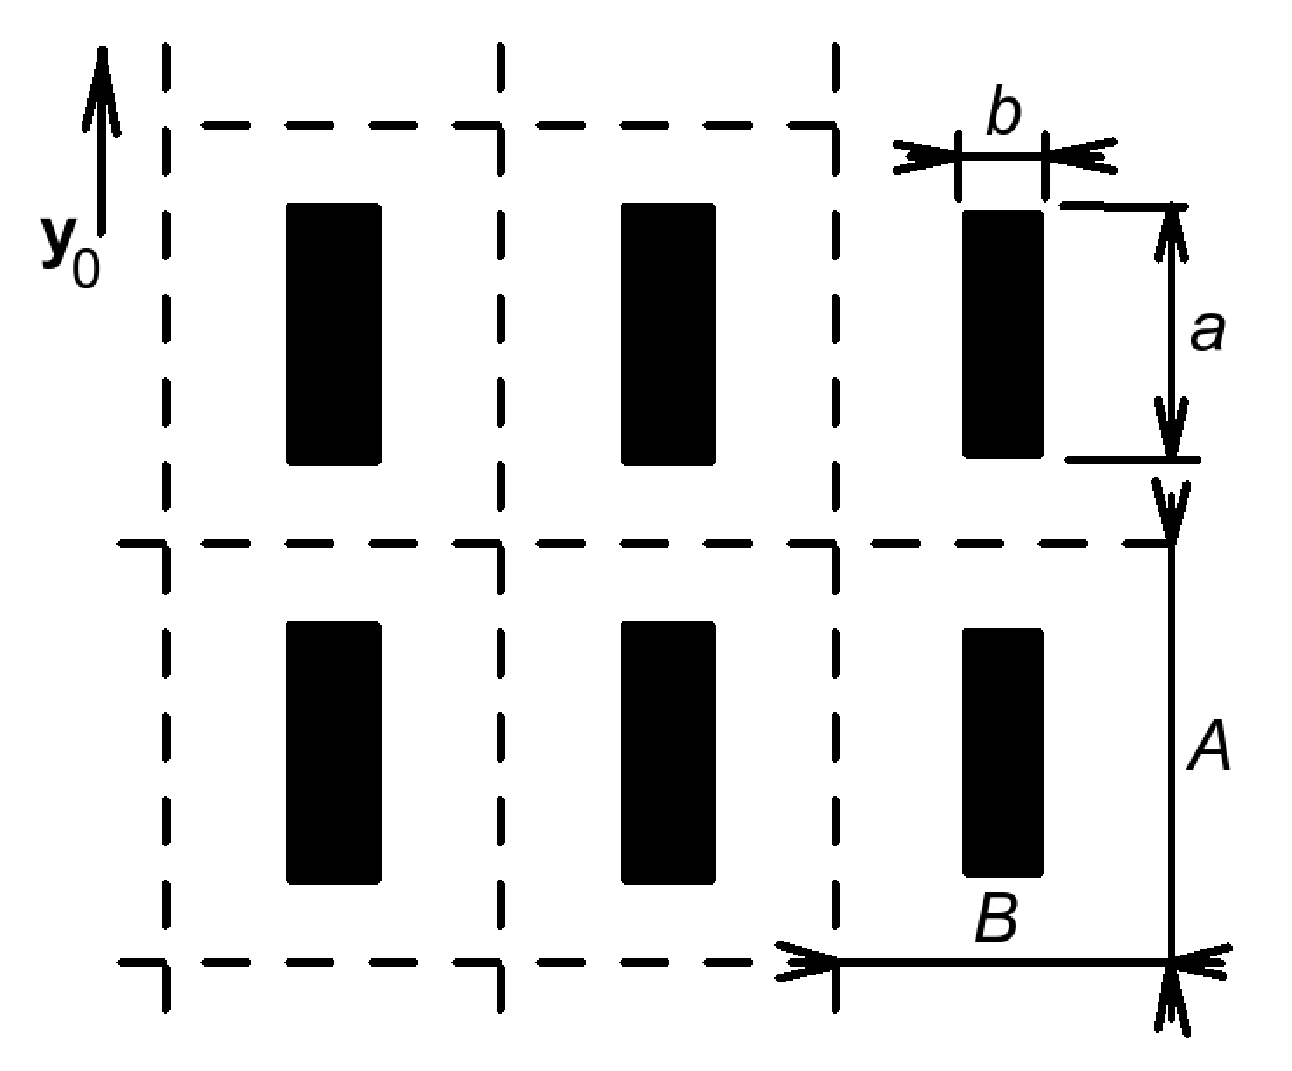
\includegraphics{obr1.eps}}
%\input{obr/dr1a.pstex_t}
\caption{The description of a figure is of the same style as the description of a table; the figure itself is of the environment \texttt{figure}.
} 
\label{fig1}
\end{center}
\end{figure}%\vspace{5mm}
%
%		example of twocolumn figure - pay attention to figure numbering, may be wrong.
%
%\begin{figure*}[ht!]
%\begin{center}
%\resizebox{65mm}{!}{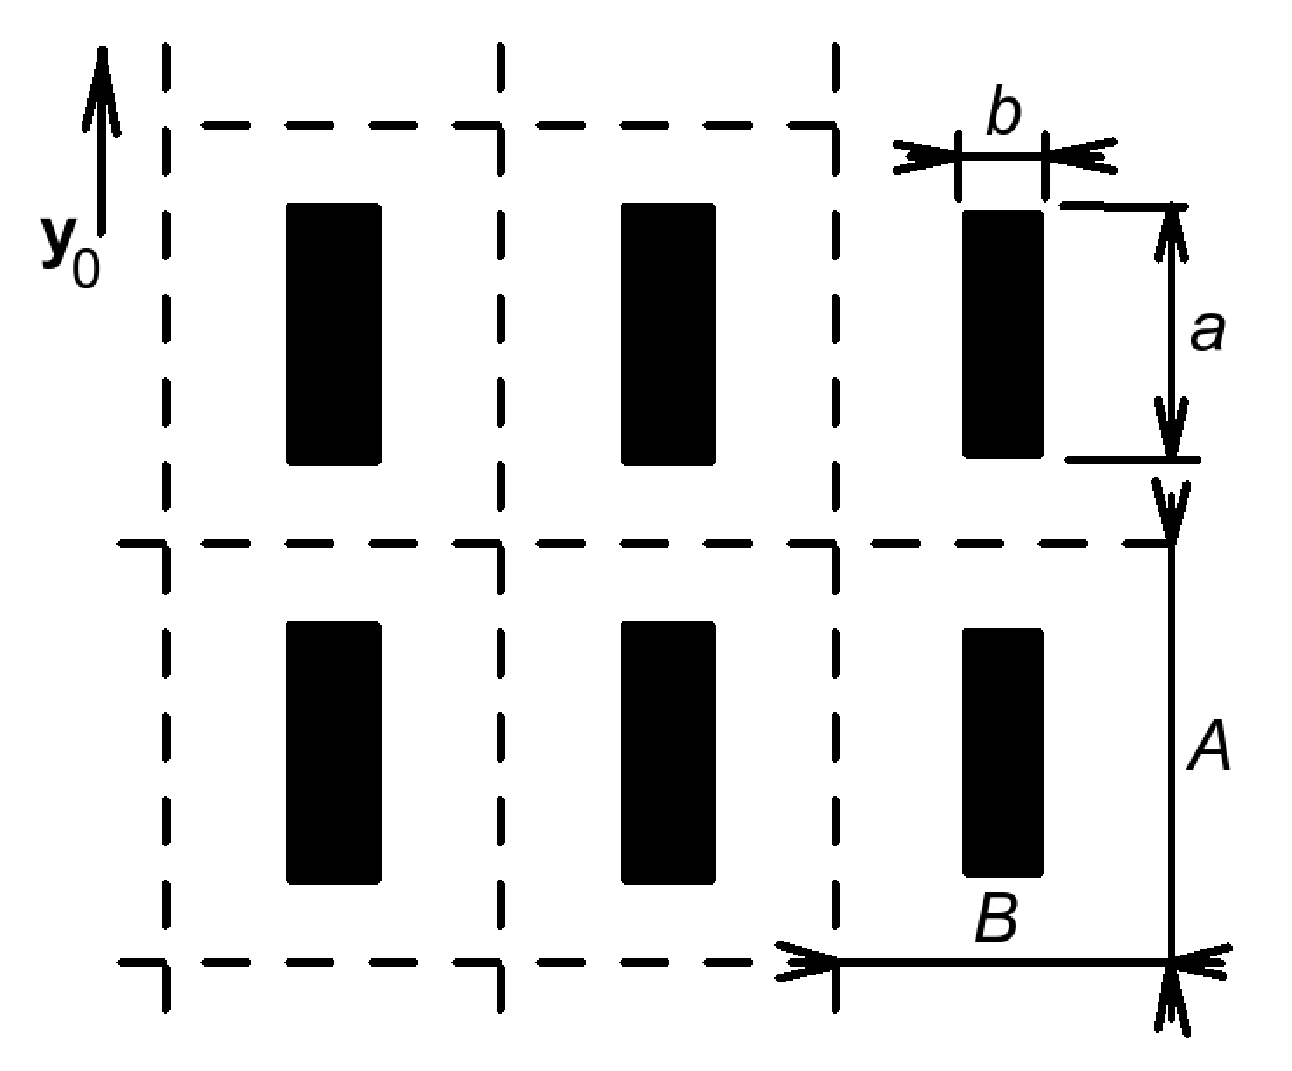
\includegraphics{obr1.eps}}
%\captionwide{The example of two-column figure and caption.
%} 
%\label{figwide}
%\end{center}
%\end{figure*}
%
\section{Headline of a Section}
Finally, we would like to ask authors for keeping the following rules:
\begin{itemize}
\item All authors must have a student status! The supervisor can be mentioned only in the \emph{Acknowledgements} section. \textbf{Failure to comply with this rule may lead to rejection of the paper}.

\item Authors are requested to submit their papers electronically to the conference web site, \textbf{which is the moment when you register for the conference}. Please, do NOT send the papers by e-mail. 

\item The file size in the pdf format (all fonts embedded) is limited to maximum 3.5 MB. Always use the up-to-date version. \textbf{Make sure that all fonts are embedded}. 

\item The length of the paper should depend on its contents (balance between the text and figures). The Program Committee will assess the completeness of the information presented. The text body of the paper itself might not exceed 5 pages. 

\item Authors are invited to include their short professional curriculum and an ID-sized photo at the end of their papers.
\end{itemize}

%----------------------------------------------------------
%               THIS IS THE PLACE FOR  ACKNOWLEDGEMENTS
\section*{Acknowledgements}
Research described in the paper was supervised by Prof. A. Supervisor, FEE CTU in Prague and supported by the Czech Grant Agency under grant No. 102/ 01/9999, by the Czech Ministry of Education under grant No. 9999/2002 and by the research program MSM 444222.

The headline \emph{Acknowledgements} is of the  style \verb+\section*{}+.

The authors are asked to pay special attention to the form of references. The NAMES OF AUTHORS should be typed in capitals, the \emph{Titles of Journals, Books or Proceedings} in italics with the first capital letter in all significant words. The tittles of articles are typed similarly as the basic text without the first capital letter in all words. Use the standart environment \verb+thebibliography+.

%----------------------------------------------------------
%               THIS IS THE PLACE FOR REFERENCES
\begin{thebibliography}{9}
\bibitem{paper}
JAKUBOV\'A, I., RAIDA, Z. Exemplary Document for the paper in Radioengineering. \emph{Radioengineering}, 2006, vol. 15, no. 1, p. 1 - 2.
\bibitem{book}
AUTHOR, F., AUTHOR, S., AUTHOR, T. F. \emph{The Book}. 2nd ed. Humpolec: Nupish\&Publish, 1901.
\bibitem{article}
HUSN\'IK, L., LHOTSK\'A, L. About Poster 2005. In \emph{Proceedings of the 9th International Student Conference on Electrical Engineering POSTER 2005}. Prague (Czech Republic), 2005, p. 1 - 2.
\end{thebibliography}


%----------------------------------------------------------
%               THIS IS THE PLACE FOR AUTHOR CV
\begin{authorcv}{First AUTHOR}
was born in \dots The biography is typed using the environment \verb+authorcv{First AUTHOR}+. 

For one author, one paragraph of the biography is devoted. The \textbf{Name} of the author is typed in  \verb+\textbf{}+, the \textbf{SURNAME} is written in capitals.  All authors must have a student status!
\end{authorcv}

\end{document}
